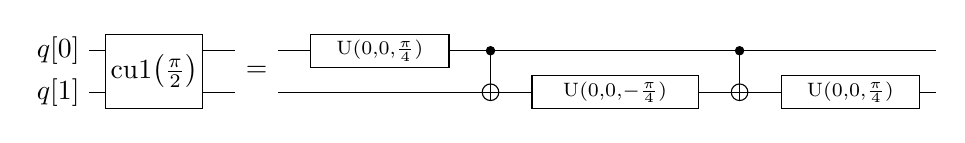
\begin{tikzpicture}[scale=1.000000,x=1pt,y=1pt]
\filldraw[color=white] (0.000000, -7.500000) rectangle (306.000000, 22.500000);
% Drawing wires
% Line 1: q0 W q[0]
\draw[color=black] (0.000000,15.000000) -- (306.000000,15.000000);
\draw[color=black] (0.000000,15.000000) node[left] {$q[0]$};
% Line 2: q1 W q[1]
\draw[color=black] (0.000000,0.000000) -- (306.000000,0.000000);
\draw[color=black] (0.000000,0.000000) node[left] {$q[1]$};
% Done with wires; drawing gates
% Line 3: q0 q1 G {cu1$\left(\frac{\pi}{2}\right)$} width=35
\draw (23.500000,15.000000) -- (23.500000,0.000000);
\begin{scope}
\draw[fill=white] (23.500000, 7.500000) +(-45.000000:24.748737pt and 19.091883pt) -- +(45.000000:24.748737pt and 19.091883pt) -- +(135.000000:24.748737pt and 19.091883pt) -- +(225.000000:24.748737pt and 19.091883pt) -- cycle;
\clip (23.500000, 7.500000) +(-45.000000:24.748737pt and 19.091883pt) -- +(45.000000:24.748737pt and 19.091883pt) -- +(135.000000:24.748737pt and 19.091883pt) -- +(225.000000:24.748737pt and 19.091883pt) -- cycle;
\draw (23.500000, 7.500000) node {{cu1$\left(\frac{\pi}{2}\right)$}};
\end{scope}
% Line 4: =
\draw[fill=white,color=white] (53.000000, -6.000000) rectangle (68.000000, 21.000000);
\draw (60.500000, 7.500000) node {$=$};
% Line 5: q0 G {U(0,0,$\frac{\pi}{4}$)} width=50
\begin{scope}
\draw[fill=white] (105.000000, 15.000000) +(-45.000000:35.355339pt and 8.485281pt) -- +(45.000000:35.355339pt and 8.485281pt) -- +(135.000000:35.355339pt and 8.485281pt) -- +(225.000000:35.355339pt and 8.485281pt) -- cycle;
\clip (105.000000, 15.000000) +(-45.000000:35.355339pt and 8.485281pt) -- +(45.000000:35.355339pt and 8.485281pt) -- +(135.000000:35.355339pt and 8.485281pt) -- +(225.000000:35.355339pt and 8.485281pt) -- cycle;
\draw (105.000000, 15.000000) node {\scriptsize{U(0,0,$\frac{\pi}{4}$)}};
\end{scope}
% Line 6: q0 +q1
\draw (145.000000,15.000000) -- (145.000000,0.000000);
\filldraw (145.000000, 15.000000) circle(1.500000pt);
\begin{scope}
\draw[fill=white] (145.000000, 0.000000) circle(3.000000pt);
\clip (145.000000, 0.000000) circle(3.000000pt);
\draw (142.000000, 0.000000) -- (148.000000, 0.000000);
\draw (145.000000, -3.000000) -- (145.000000, 3.000000);
\end{scope}
% Line 7: q1 G {U(0,0,$-\frac{\pi}{4}$)} width=60
\begin{scope}
\draw[fill=white] (190.000000, -0.000000) +(-45.000000:42.426407pt and 8.485281pt) -- +(45.000000:42.426407pt and 8.485281pt) -- +(135.000000:42.426407pt and 8.485281pt) -- +(225.000000:42.426407pt and 8.485281pt) -- cycle;
\clip (190.000000, -0.000000) +(-45.000000:42.426407pt and 8.485281pt) -- +(45.000000:42.426407pt and 8.485281pt) -- +(135.000000:42.426407pt and 8.485281pt) -- +(225.000000:42.426407pt and 8.485281pt) -- cycle;
\draw (190.000000, -0.000000) node {\scriptsize{U(0,0,$-\frac{\pi}{4}$)}};
\end{scope}
% Line 8: q0 +q1
\draw (235.000000,15.000000) -- (235.000000,0.000000);
\filldraw (235.000000, 15.000000) circle(1.500000pt);
\begin{scope}
\draw[fill=white] (235.000000, 0.000000) circle(3.000000pt);
\clip (235.000000, 0.000000) circle(3.000000pt);
\draw (232.000000, 0.000000) -- (238.000000, 0.000000);
\draw (235.000000, -3.000000) -- (235.000000, 3.000000);
\end{scope}
% Line 9: q1 G {U(0,0,$\frac{\pi}{4}$)} width=50
\begin{scope}
\draw[fill=white] (275.000000, -0.000000) +(-45.000000:35.355339pt and 8.485281pt) -- +(45.000000:35.355339pt and 8.485281pt) -- +(135.000000:35.355339pt and 8.485281pt) -- +(225.000000:35.355339pt and 8.485281pt) -- cycle;
\clip (275.000000, -0.000000) +(-45.000000:35.355339pt and 8.485281pt) -- +(45.000000:35.355339pt and 8.485281pt) -- +(135.000000:35.355339pt and 8.485281pt) -- +(225.000000:35.355339pt and 8.485281pt) -- cycle;
\draw (275.000000, -0.000000) node {\scriptsize{U(0,0,$\frac{\pi}{4}$)}};
\end{scope}
% Done with gates; drawing ending labels
% Done with ending labels; drawing cut lines and comments
% Done with comments
\end{tikzpicture}
